\subsection{Análisis de Fronteras de Nyquist y Restricciones de Simulación}
La simulación en radiofrecuencia (RF) impone una carga computacional superior a la Envolvente Compleja (EC) debido a que la portadora ($f_c$) eleva la frecuencia máxima del sistema, exigiendo una tasa de muestras por símbolo (SPS) que garantice $f_s > 2f_{max}$. 

A partir del criterio de Nyquist-Shannon, se determinaron analíticamente los límites operativos para los parámetros por defecto ($f_s = 4.096$ MHz, $R_s = 32$ kHz):
\begin{itemize}
    \item \textbf{Límite de Portadora en RF:} $f_{c\_max} \le \frac{f_s}{2} - f_d = 2.016$ MHz[cite: 320].
    \item \textbf{Límite de Desviación en EC:} $f_d \le \frac{f_s}{2} = 2.048$ MHz[cite: 326].
    \item \textbf{SPS Mínimo para BPSK en RF:} Basado en $f_s \ge 2(f_c + R_s)$, se deduce $SPS_{min} \ge \frac{2f_c}{R_s} + 2$, lo que para $f_c = 128$ kHz resulta en $SPS_{min} \ge 10$.
\end{itemize}

La validez del diseño del VCO se comprueba en la Figura \ref{fig:resultados_vco}. En el dominio del tiempo, se observa una resolución continua de la sinusoide, mientras que el espectro permanece libre de \textit{aliasing} ruidoso\cite{gnuradio}. 

\begin{figure}[H]
    \centering
    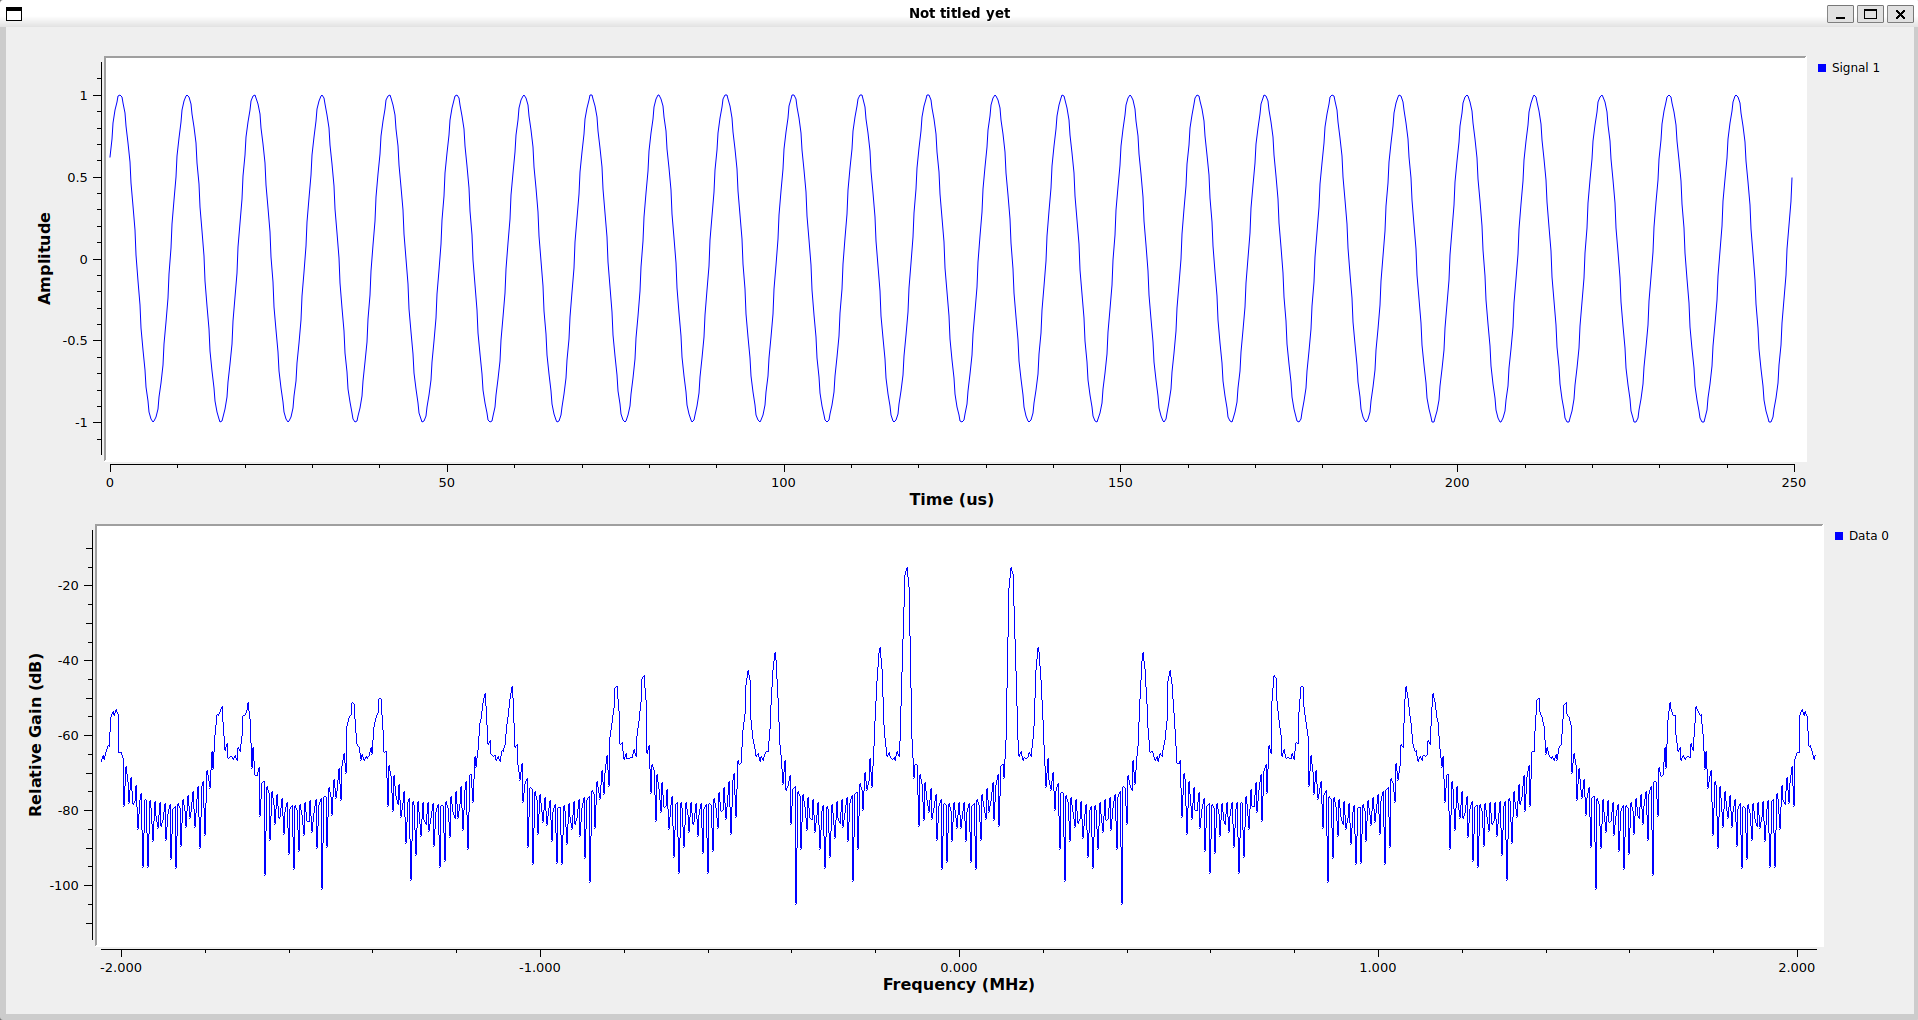
\includegraphics[width=0.95\linewidth]{imagenes/prueba.png}
    \caption{Validación experimental: (a) Señal modulada en tiempo y (b) Densidad espectral de potencia.}
    \label{fig:resultados_vco}
\end{figure}

Finalmente, se determinó que la ubicación del filtro interpolador es crítica en FSK. A diferencia de BPSK, donde el escalado y el filtrado son conmutativos por linealidad LTI, en FSK el filtrado debe preceder a la integración para evitar picos transitorios y distorsiones en la derivada de la fase que comprometerían los saltos frecuenciales.